\documentclass[12pt,parskip=full]{article}
\usepackage{lmodern}
\usepackage{amsmath}
\usepackage[left=1.0in,right=1.0in,top=0.5in,bottom=1.0in]{geometry}
\geometry{letterpaper}
\usepackage{graphicx}
\usepackage{caption}
\usepackage{subcaption}
\usepackage{longtable}
\usepackage{float}
\usepackage{wrapfig}
\usepackage{soul}
\usepackage{textcomp}
\usepackage{marvosym}
\usepackage{wasysym}
\usepackage{latexsym}
\usepackage{amssymb}
\usepackage{apacite}
\usepackage{tabu}
\usepackage[svgnames]{xcolor}
\usepackage{tikz}
\usepackage[linktoc=all]{hyperref}
\usepackage{cleveref}
\usepackage{listings}
\usepackage{setspace}
\usepackage{parskip}
\usepackage{array}
\usepackage{apacite}
\usepackage{natbib}
\usepackage{multicol}
\usepackage{subcaption}
\usepackage{mathtools}
\usetikzlibrary{arrows}

\pgfdeclarelayer{edgelayer}
\pgfdeclarelayer{nodelayer}
\pgfsetlayers{edgelayer,nodelayer,main}

\tikzstyle{none}=[inner sep=0pt]
\tikzstyle{waypt}=[circle,fill=Black,draw=Black,scale=0.4]
\tikzstyle{Helobody}=[circle,fill=White,draw=Black,scale=4.0]
\tikzstyle{Tailrotor}=[circle,fill=White,draw=Black,scale=1.0]
\tikzstyle{ForceVector}=[->,draw=Indigo,fill=Indigo]
\tikzstyle{Coordinate}=[->,draw=Red,fill=Red,fill opacity=1.0]
\tikzstyle{angle}=[->]
\tikzstyle{MeasureMark}=[|-|]
\newlength{\imagewidth}
\newlength{\imagescale}

\setlength{\parskip}{11pt}
%\setlength{\parindent}{15pt}
\usepackage{bookmark}
\makeatletter
%\renewcommand\@seccntformat[1]{}
\makeatother

\lstset
{
	language=c,
	keywords={break,case,catch,continue,else,for,
		if,return,switch,try,while,int,void},
	basicstyle=\ttfamily,
	keywordstyle=\color{blue},
	commentstyle=\color{ForestGreen},
	stringstyle=\color{purple},
	numbers=left,
	numberstyle=\tiny\color{gray},
	stepnumber=1,
	numbersep=10pt,
	backgroundcolor=\color{white},
	tabsize=4,
	showspaces=false,
	showstringspaces=false
}

\renewcommand{\thesection}{\arabic{section}}

\renewcommand{\thesubsection}{\thesection\alph{subsection}}
\renewcommand{\theequation}{\thesubsection\arabic{equation}}
\newcommand*\circled[1]{\tikz[baseline=(char.base)]{
			\node[shape=circle,draw,inner sep=1pt] (char) {#1};}}
			
\numberwithin{subsection}{section}

\begin{document}
	\vspace{-4ex}
	\title{EbbCFD Theory Guide\vspace{-3.5ex}}
	\author{Rob Rau\vspace{-4ex}}
	\date{\today\vspace{-4ex}}
	\maketitle

	\section{Introduction}
		EbbCFD is a computational fluid dynamics package intended to solve the compressible Euler equations.
		It uses an unstructured, limited, second order finite volume spacial scheme and supports numerous
		time integration schemes. This document covers the theory behind EbbCFD's implementation

	\section{Unstructured Finite Volume}
		EbbCFD operates on completely unstructured meshes. In theory it supports cell geometries of up to six faces,
		though only triangular meshes have been extensively tested. For a first order spatial update, the numerical flux
		is computed on each edge in the mesh, than, for each cell in the mesh, those fluxes are summed and called the
		flux residuals.
		\begin{equation}
			\mathbf{R}_i = \sum_{e = 1}^{N_{f_i}}{m\mathbf{\hat{F}}(\mathbf{U}_i, \mathbf{U}_{N(i,e)}, \vec{n}_{i,e}) \Delta l_{i,e}}
		\end{equation}
		where $\mathbf{\hat{F}}(\mathbf{U}_i, \mathbf{U}_{N(i,e)}, \vec{n}_{i,e})$ is the numerical flux function,
		$\Delta l_{i,e}$ is the length of the cell edge, $N_{f_i}$ is the number of faces of cell $i$, and $m$ is $\pm 1$
		depending on which cell the normal $\vec{n}_{i,e}$ belonged to. This possible because the flux function is homogeneous, i.e.
		$\mathbf{\hat{F}}(\mathbf{U}_i, \mathbf{U}_{N(i,e)}, \vec{n}_{i,e}) = -\mathbf{\hat{F}}(\mathbf{U}_i, \mathbf{U}_{N(i,e)}, -\vec{n}_{i,e})$.
		This allows the code to compute the flux only once per edge, and then depending on the cell, multiply by $\pm 1$.
		With this flux residual we can write the semi-discrete form of the first order finite volume update.
		\begin{equation}
			\frac{\partial \mathbf{U}_i}{\partial t} = -\frac{1}{A_i}\mathbf{R}_i
		\end{equation}
		where $A_i$ is the area of cell $i$. Currently, EbbCFD only supports the Roe flux function, but others are planned.

	\section{Second Order}
		To achieve second order accuracy, the numerical flux is no longer computed using cell averaged state values.
		Instead, the edge state values are computed and used. To obtain edge state values, an estimate of the cell gradients 
		is necessary. To reduce solution oscillations at discontinuities in the flow, EbbCFD also supports a couple of
		different schemes for gradient limiting.

		\subsection{Gradients}
			To estimate cell gradients a least squares approximation was used. The least squares problem is set up like so
			\begin{equation}
				\mathbf{r} = \begin{bmatrix} x_1 - x_M & y_1 - y_M \\ \vdots & \vdots \\ x_{N_{f_i}} - x_M & y_{N_{f_i}} - y_M \end{bmatrix} \begin{bmatrix}D_x \\ D_y \end{bmatrix} - \begin{bmatrix} u_1 - u_M \\ \vdots \\ u_{N_{f_i}} - u_M \end{bmatrix}
			\end{equation}
			where $x_M$ and $y_M$ are the current cell centroid coordinates, $x_1..x_{N_{f_i}}$ and $y_1..y_{N_{f_i}}$ 
			are the cell centroid coordinates for the neighboring cells, $u_M$ is a conserved state variable of the current 
			cell, and $u_1..u_{N_{f_i}}$ are the conserved state variables of the neighboring cells. In 2D, four
			least squares problems need to be solved in order to get a gradient for each conserved quantity (density,
			x/y momentum, and energy for the Euler equations). For cells located at a boundary, a ghost cell approach is
			used. The cell centroid of the boundary cells is reflected across the boundary edge and its state values
			are updated in accordance with what type of boundary it is. A wall boundary for instance, will reflect the
			flow momentum across the boundary in order to cancel out the normal momentum component.

		\subsection{Limiters}
			EbbCFD currently supports two different limiting techniques. The first is a scalar limiter, where a single scalar
			value limits both x and y components of a gradient. The other is a vector limiter, where x and y gradient components
			are limited separately. Both scalar and vector limiters used in EbbCFD are implementations of ideas laid out by
			May and Berger. Specifically EbbCFD uses what is referred to as the \textit{relaxed formulation} as its gradient 
			limit constraints \cite{doi:10.1137/120875624}. The means the limiters must obey the following conditions
			\begin{equation}
				\min{(u_M, u_1, \dots, u_N)} \le u_M + \begin{bmatrix}(x_j - x_M)D_x \\ (y_j - y_M)D_y\end{bmatrix} \begin{bmatrix} \phi_x \\ \phi_y \end{bmatrix} \le \max{(u_M, u_1, \dots, u_N)}
			\end{equation}
			where $\phi_x$ and $\phi_y$ are the limiters. This method finds the min and max values of all neighboring cells and
			ensures that when the solution is reconstructed to the neighboring cell centroids, monotonicity constraints aren't
			violated.

			\subsubsection{Scalar limiter}
				For the scalar limiter, $\phi_x = \phi_y$. The limiter value is computed as follows
				\begin{align}
					u_r &= u_M + (x_j - x_M)D_x + (y_j - y_M)D_y \\
					s_j &= \begin{cases}
						\frac{u_{min} - u_M}{(x_j - x_M)D_x + (y_j - y_M)D_y} & \mathrm{if}\ u_r < u_{min} \\
						\frac{u_{max} - u_M}{(x_j - x_M)D_x + (y_j - y_M)D_y} & \mathrm{if}\ u_r > u_{max}
					\end{cases} \quad j = 1..N_{f_i} \\
					\phi &= \min{(s_0, \dots, s_{N_{f_i}})}
				\end{align}
				
			\subsubsection{Vector limiter}
				The vector limiting scheme presented by May and Berger frames the limiting problem as a linear programming problem.
				Basically, the goal is to minimize the limited gradient error, i.e.
				\begin{align}
					\mathrm{minimize}\quad &|D_x - \phi_x D_x| + |D_y - \phi_y D_y| \\
									=& -|D_x|\phi_x - |D_y|\phi_y
				\end{align}
				subject to the monotonicity constraints presented earlier. The algorithm EbbCFD uses to solve this linear
				programming problem is the All-inequality simplex method outlined in \cite{doi:10.1137/120875624}. The vector
				limiter is still an area of ongoing development as it currently seems to get in the way of convergence.

		\begin{figure}[H]
			\centering
			\begin{subfigure}[H]{0.6\textwidth}
				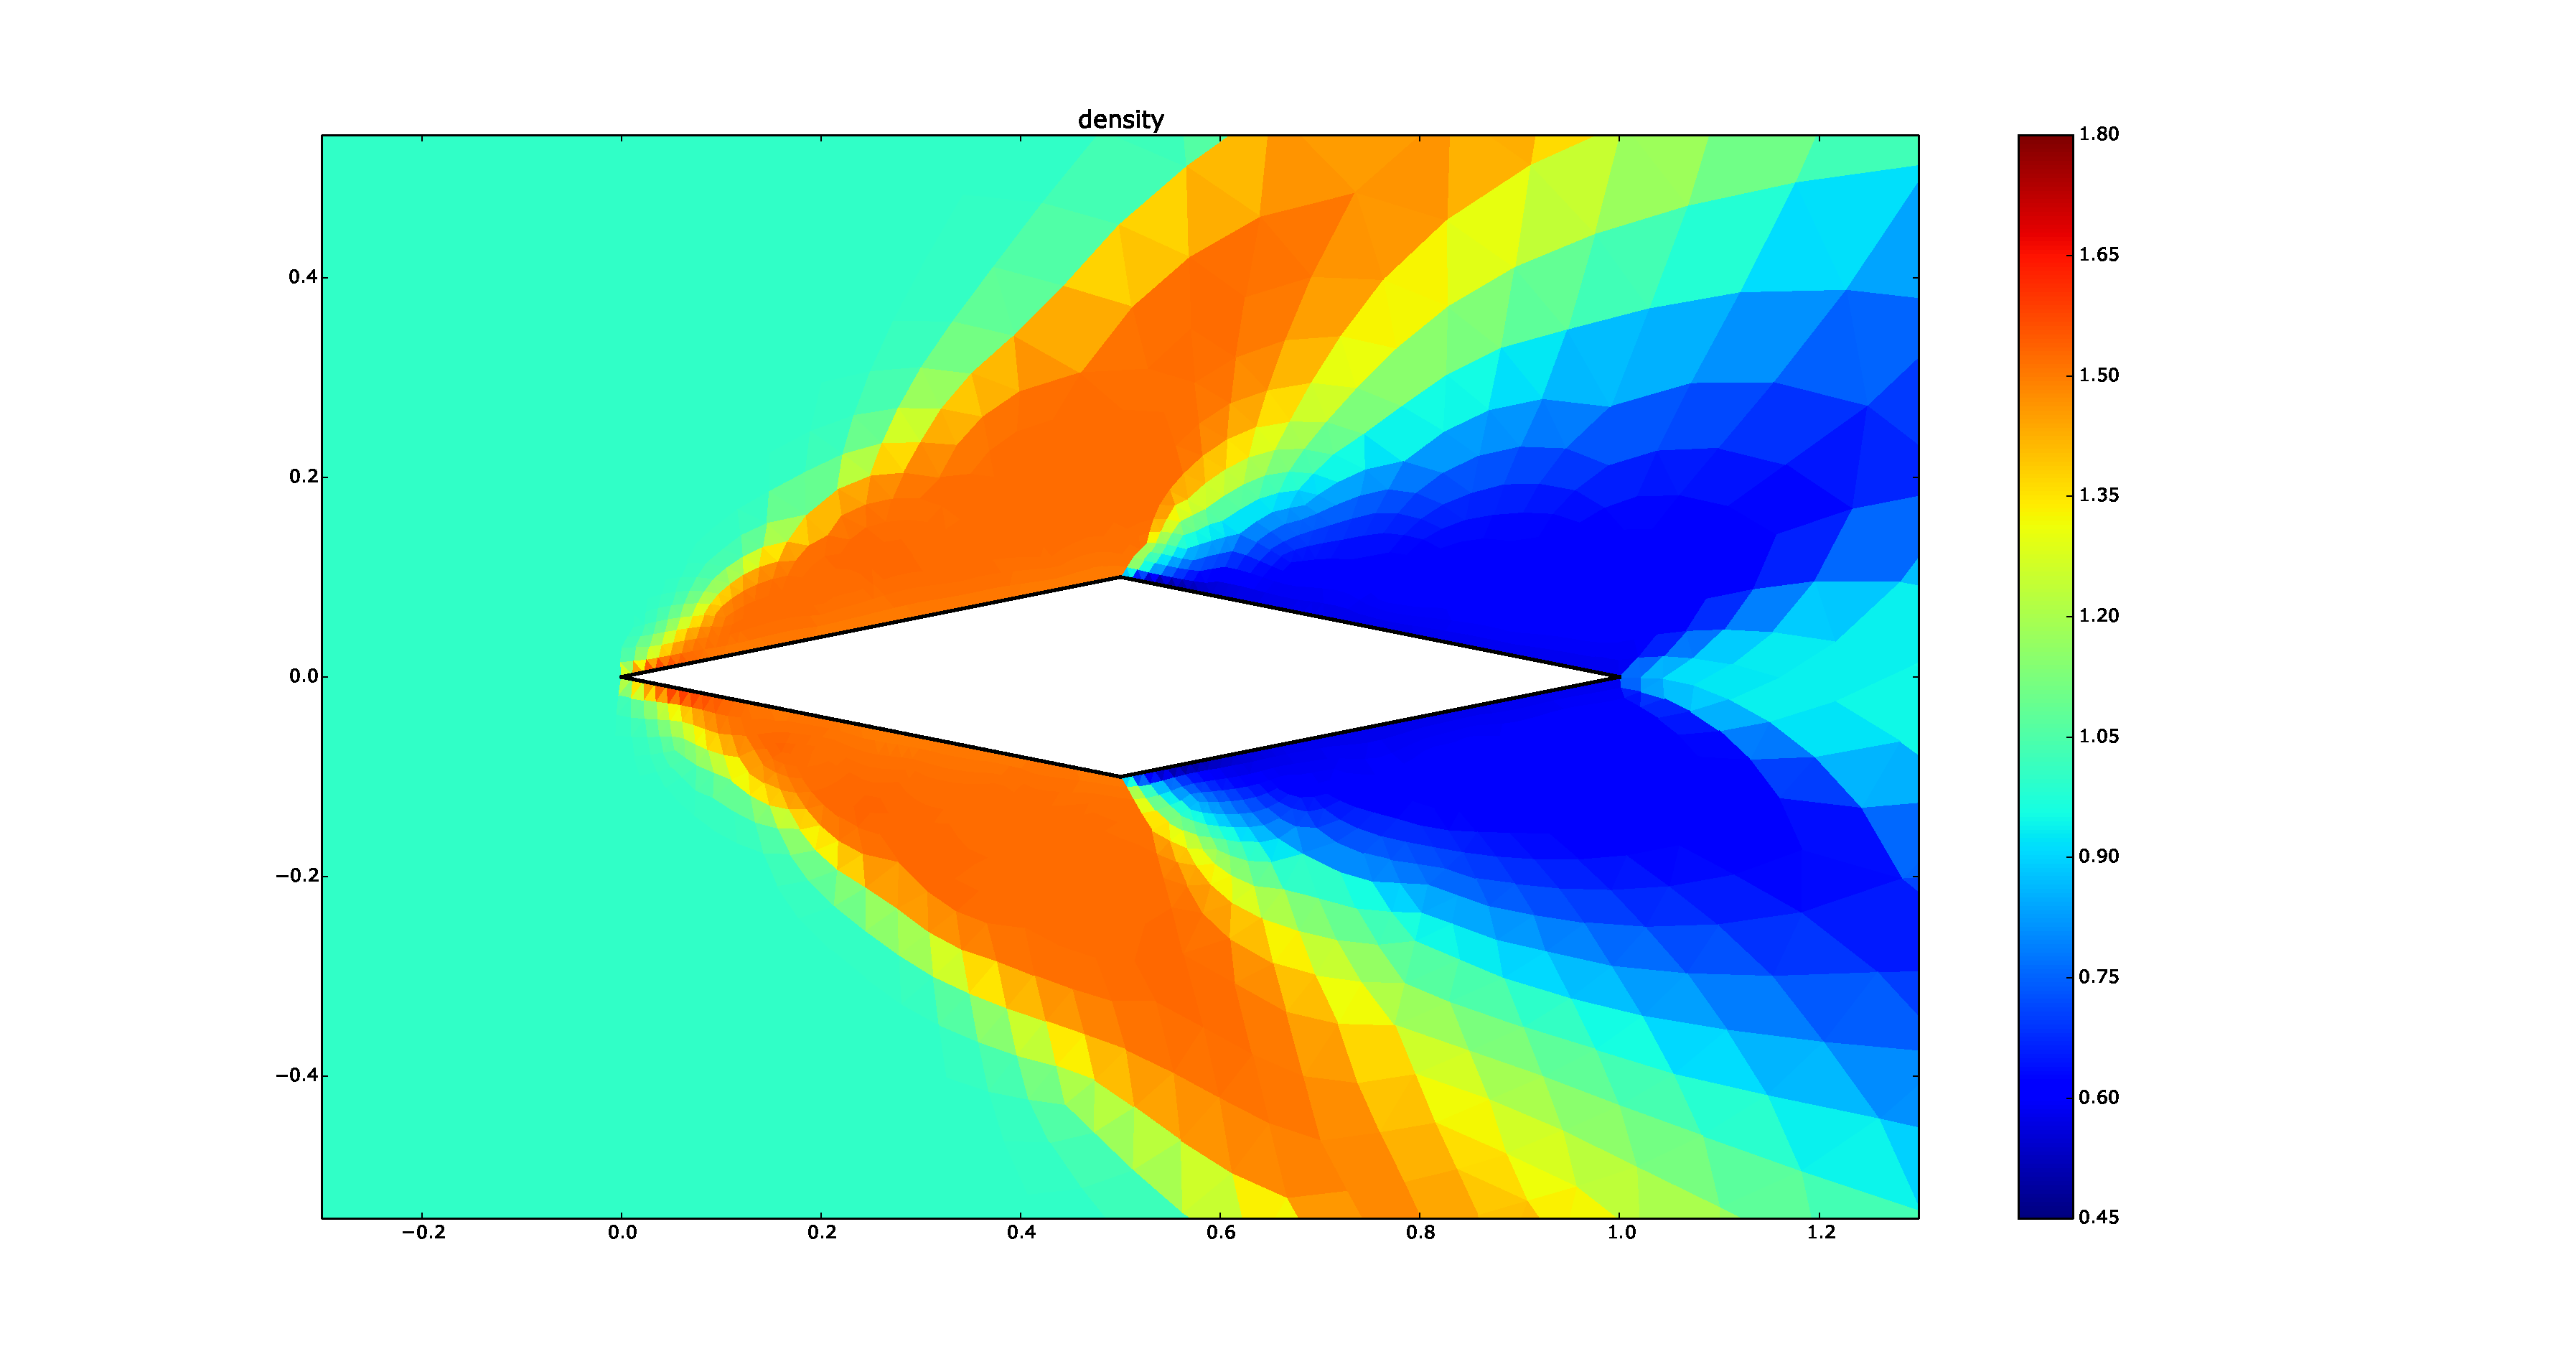
\includegraphics[width=\textwidth,trim={7cm 2cm 10cm 2cm},clip]{FirstOrderShock.pdf}
				\caption{First order shock capture}
			\end{subfigure}
			\begin{subfigure}[H]{0.6\textwidth}
				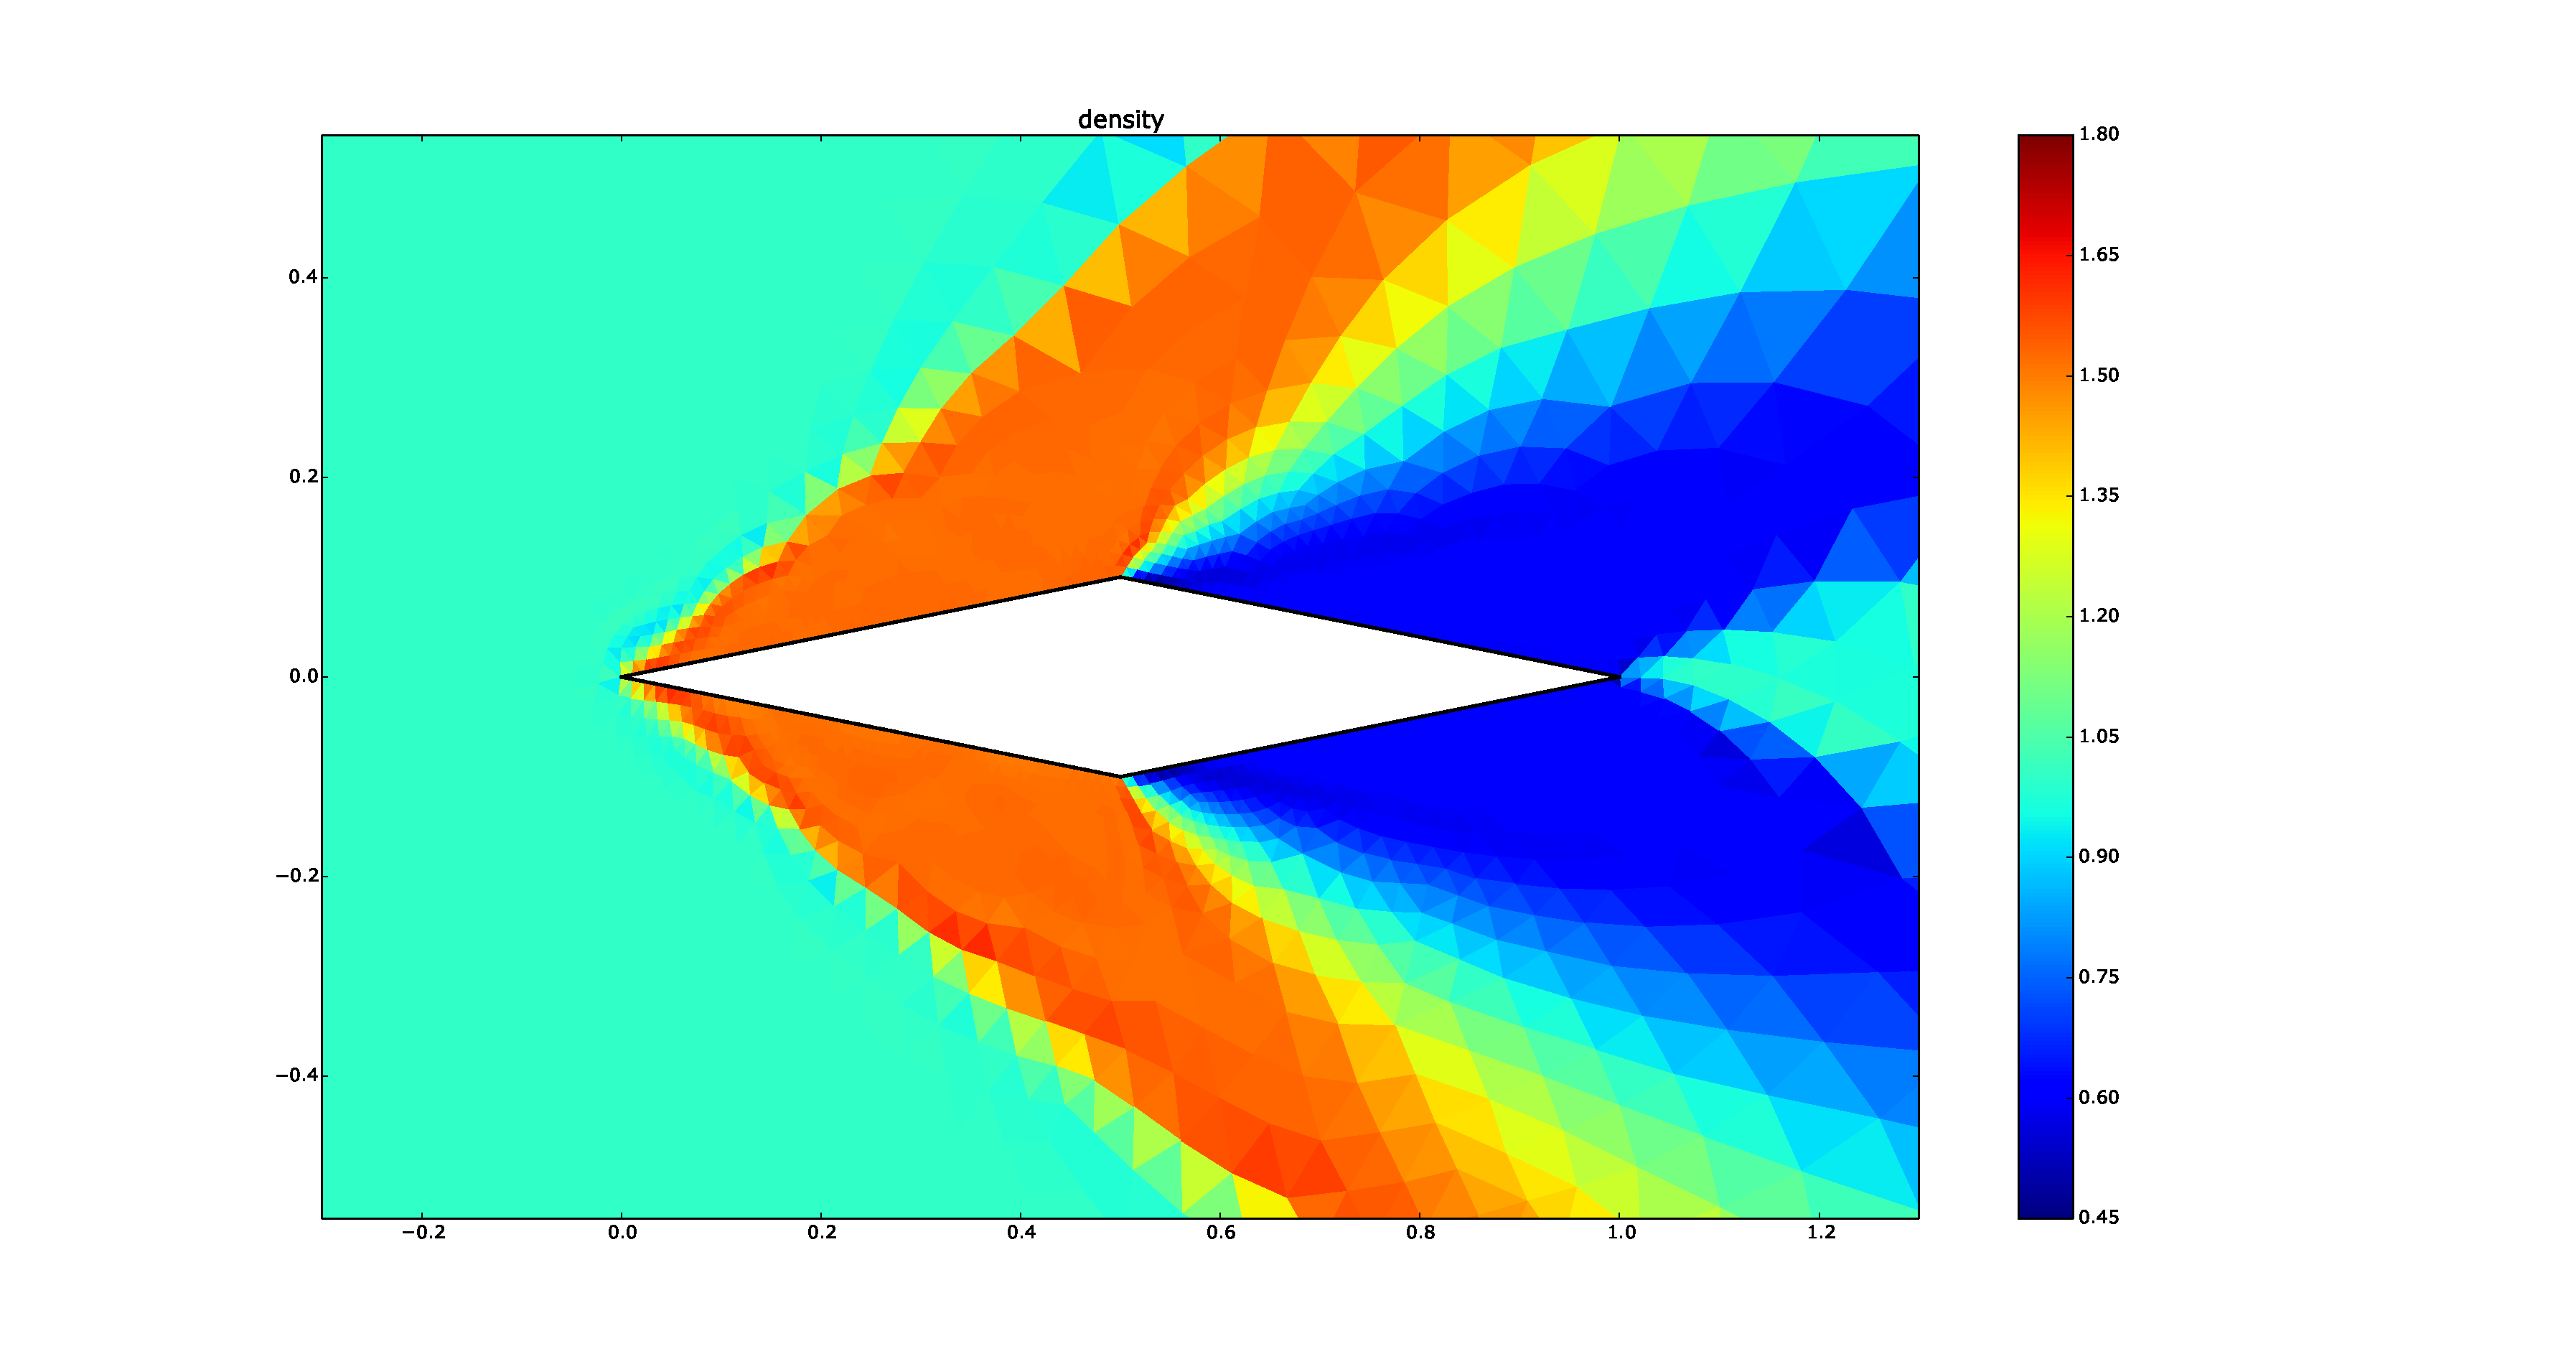
\includegraphics[width=\textwidth,trim={7cm 2cm 10cm 2cm},clip]{SecondOrderShock.pdf}
				\caption{Second order shock capture. Over/under shoot is visible at shock boundary}
			\end{subfigure}
			\begin{subfigure}[H]{0.6\textwidth}
				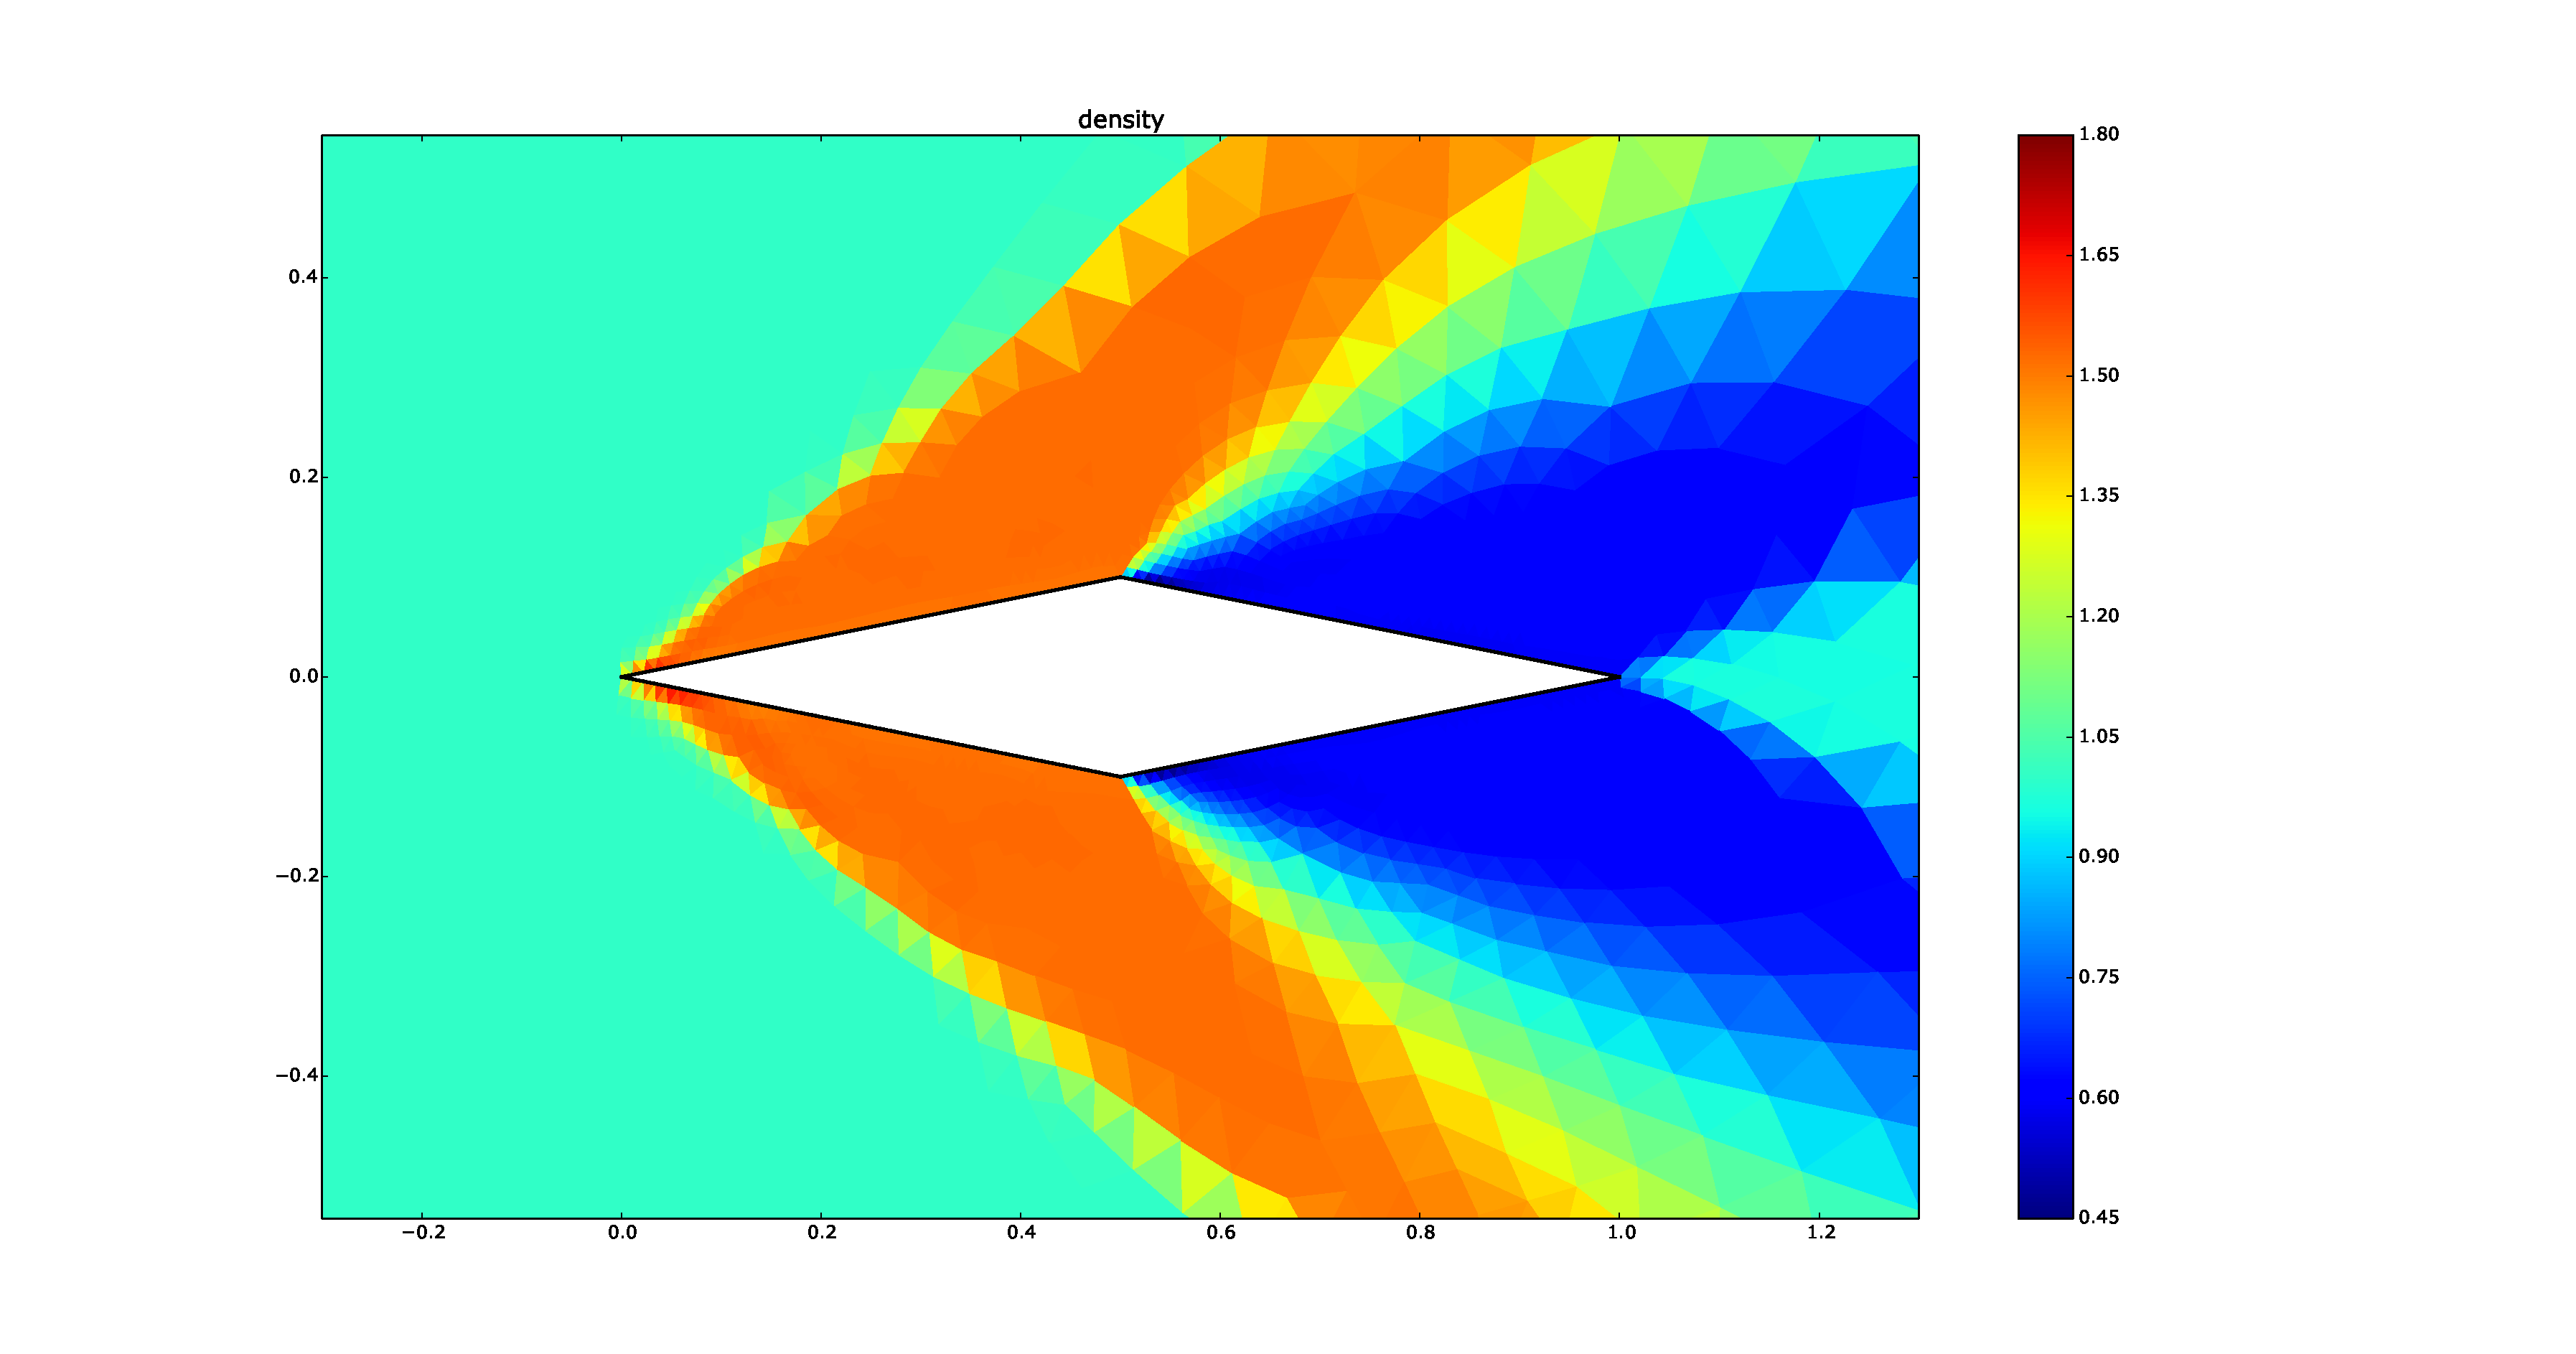
\includegraphics[width=\textwidth,trim={7cm 2cm 10cm 2cm},clip]{SecondOrderScalarLimitedShock.pdf}
				\caption{Second order with scalar limiter shock capture. Over/under shoot eliminated}
			\end{subfigure}
			\caption{Mach 2 diamond wedge airfoil}
		\end{figure}

	\section{Numerical Viscosity}
		The Euler equations neglect a dissipative term and thus are not suitable for simulating viscous flows. However, when
		discretized, the approximation of the Euler equations that are actually solved add some dissipation back into
		the solution. An attempt was made to characterize this dissipation to see if any relation between mesh size and
		viscosity could be made. The thought behind this study was to: first, at low Mach number ($M = 0.3$) generate vortices
		from the flow past a cylinder at various mesh sizes, and second, find a correlation between shedding frequency and 
		the average hydraulic diameter of the mesh.
		
		Unfortunately, EbbCFD could not be made to shed vortices around a cylinder at low Mach number, so instead a half cylinder
		was substituted. While the half cylinders did produce vortex shedding, it did not show any sort of meaningful 
		relationship between average hydraulic diameter and shedding frequency. Instead all runs snapped to one of two different
		modes as show below.

		\begin{figure}[H]
			\centering
			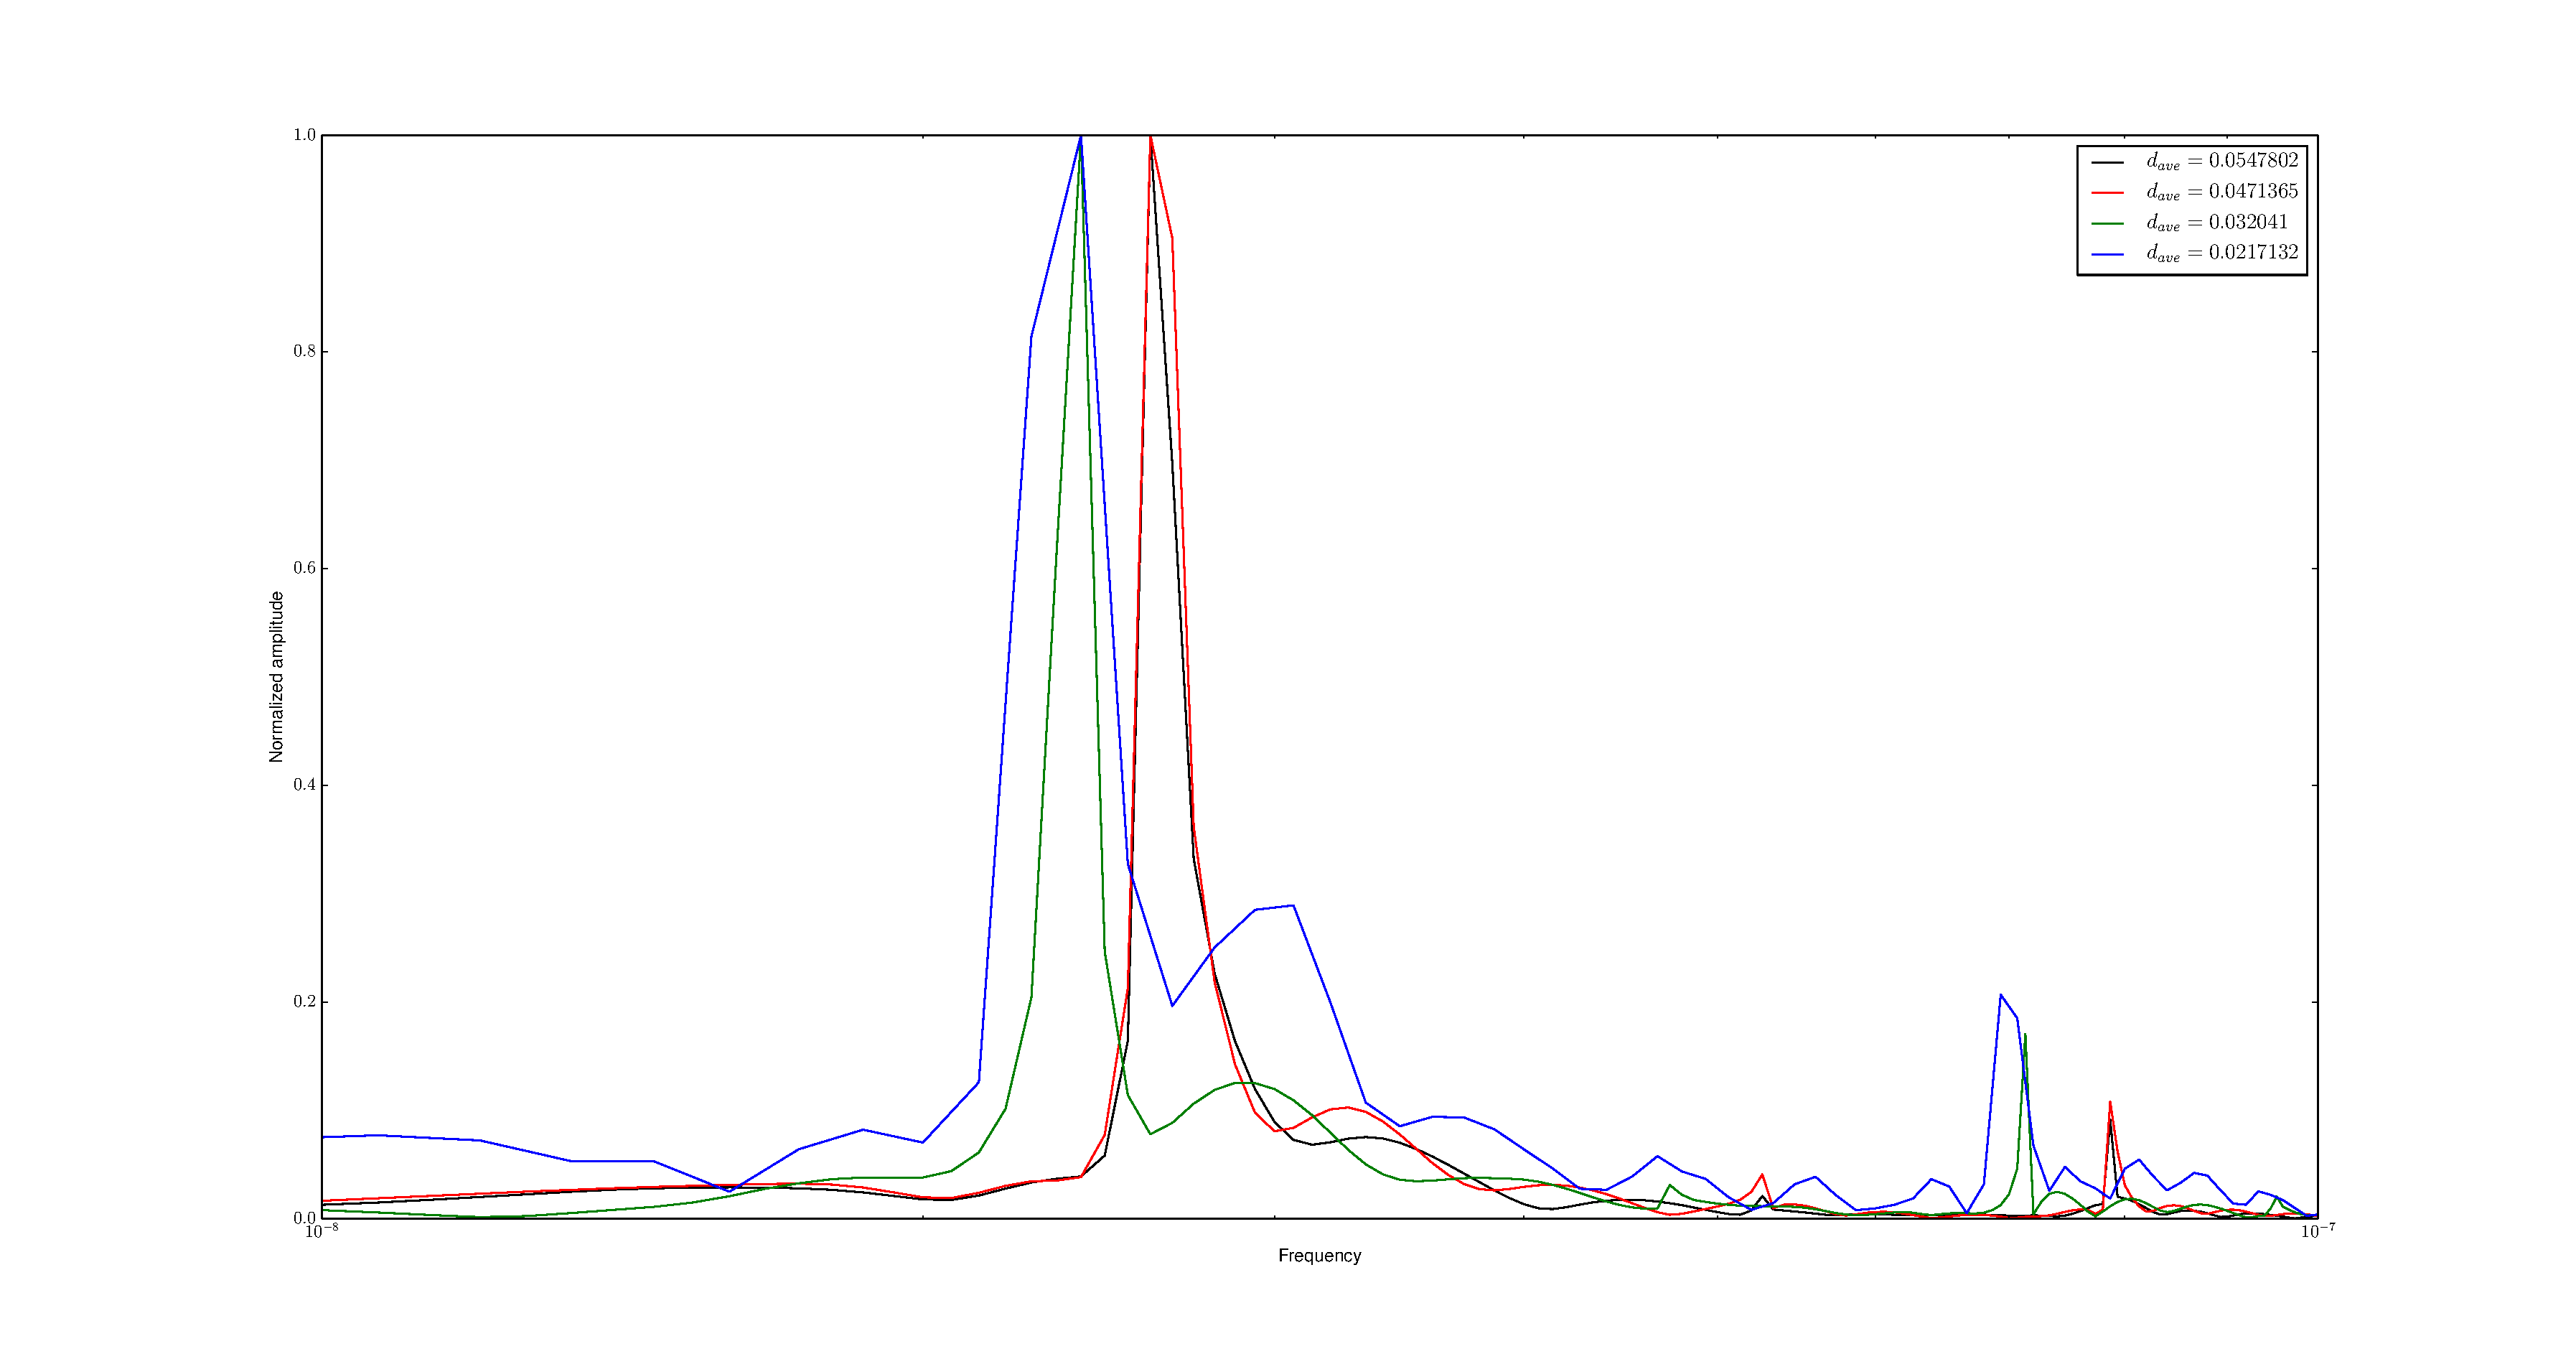
\includegraphics[width=\textwidth]{SheddingFrequency.pdf}
			\caption{Vortex shedding frequencies on different mesh sizes}
		\end{figure}
		\begin{figure}[H]
			\centering
			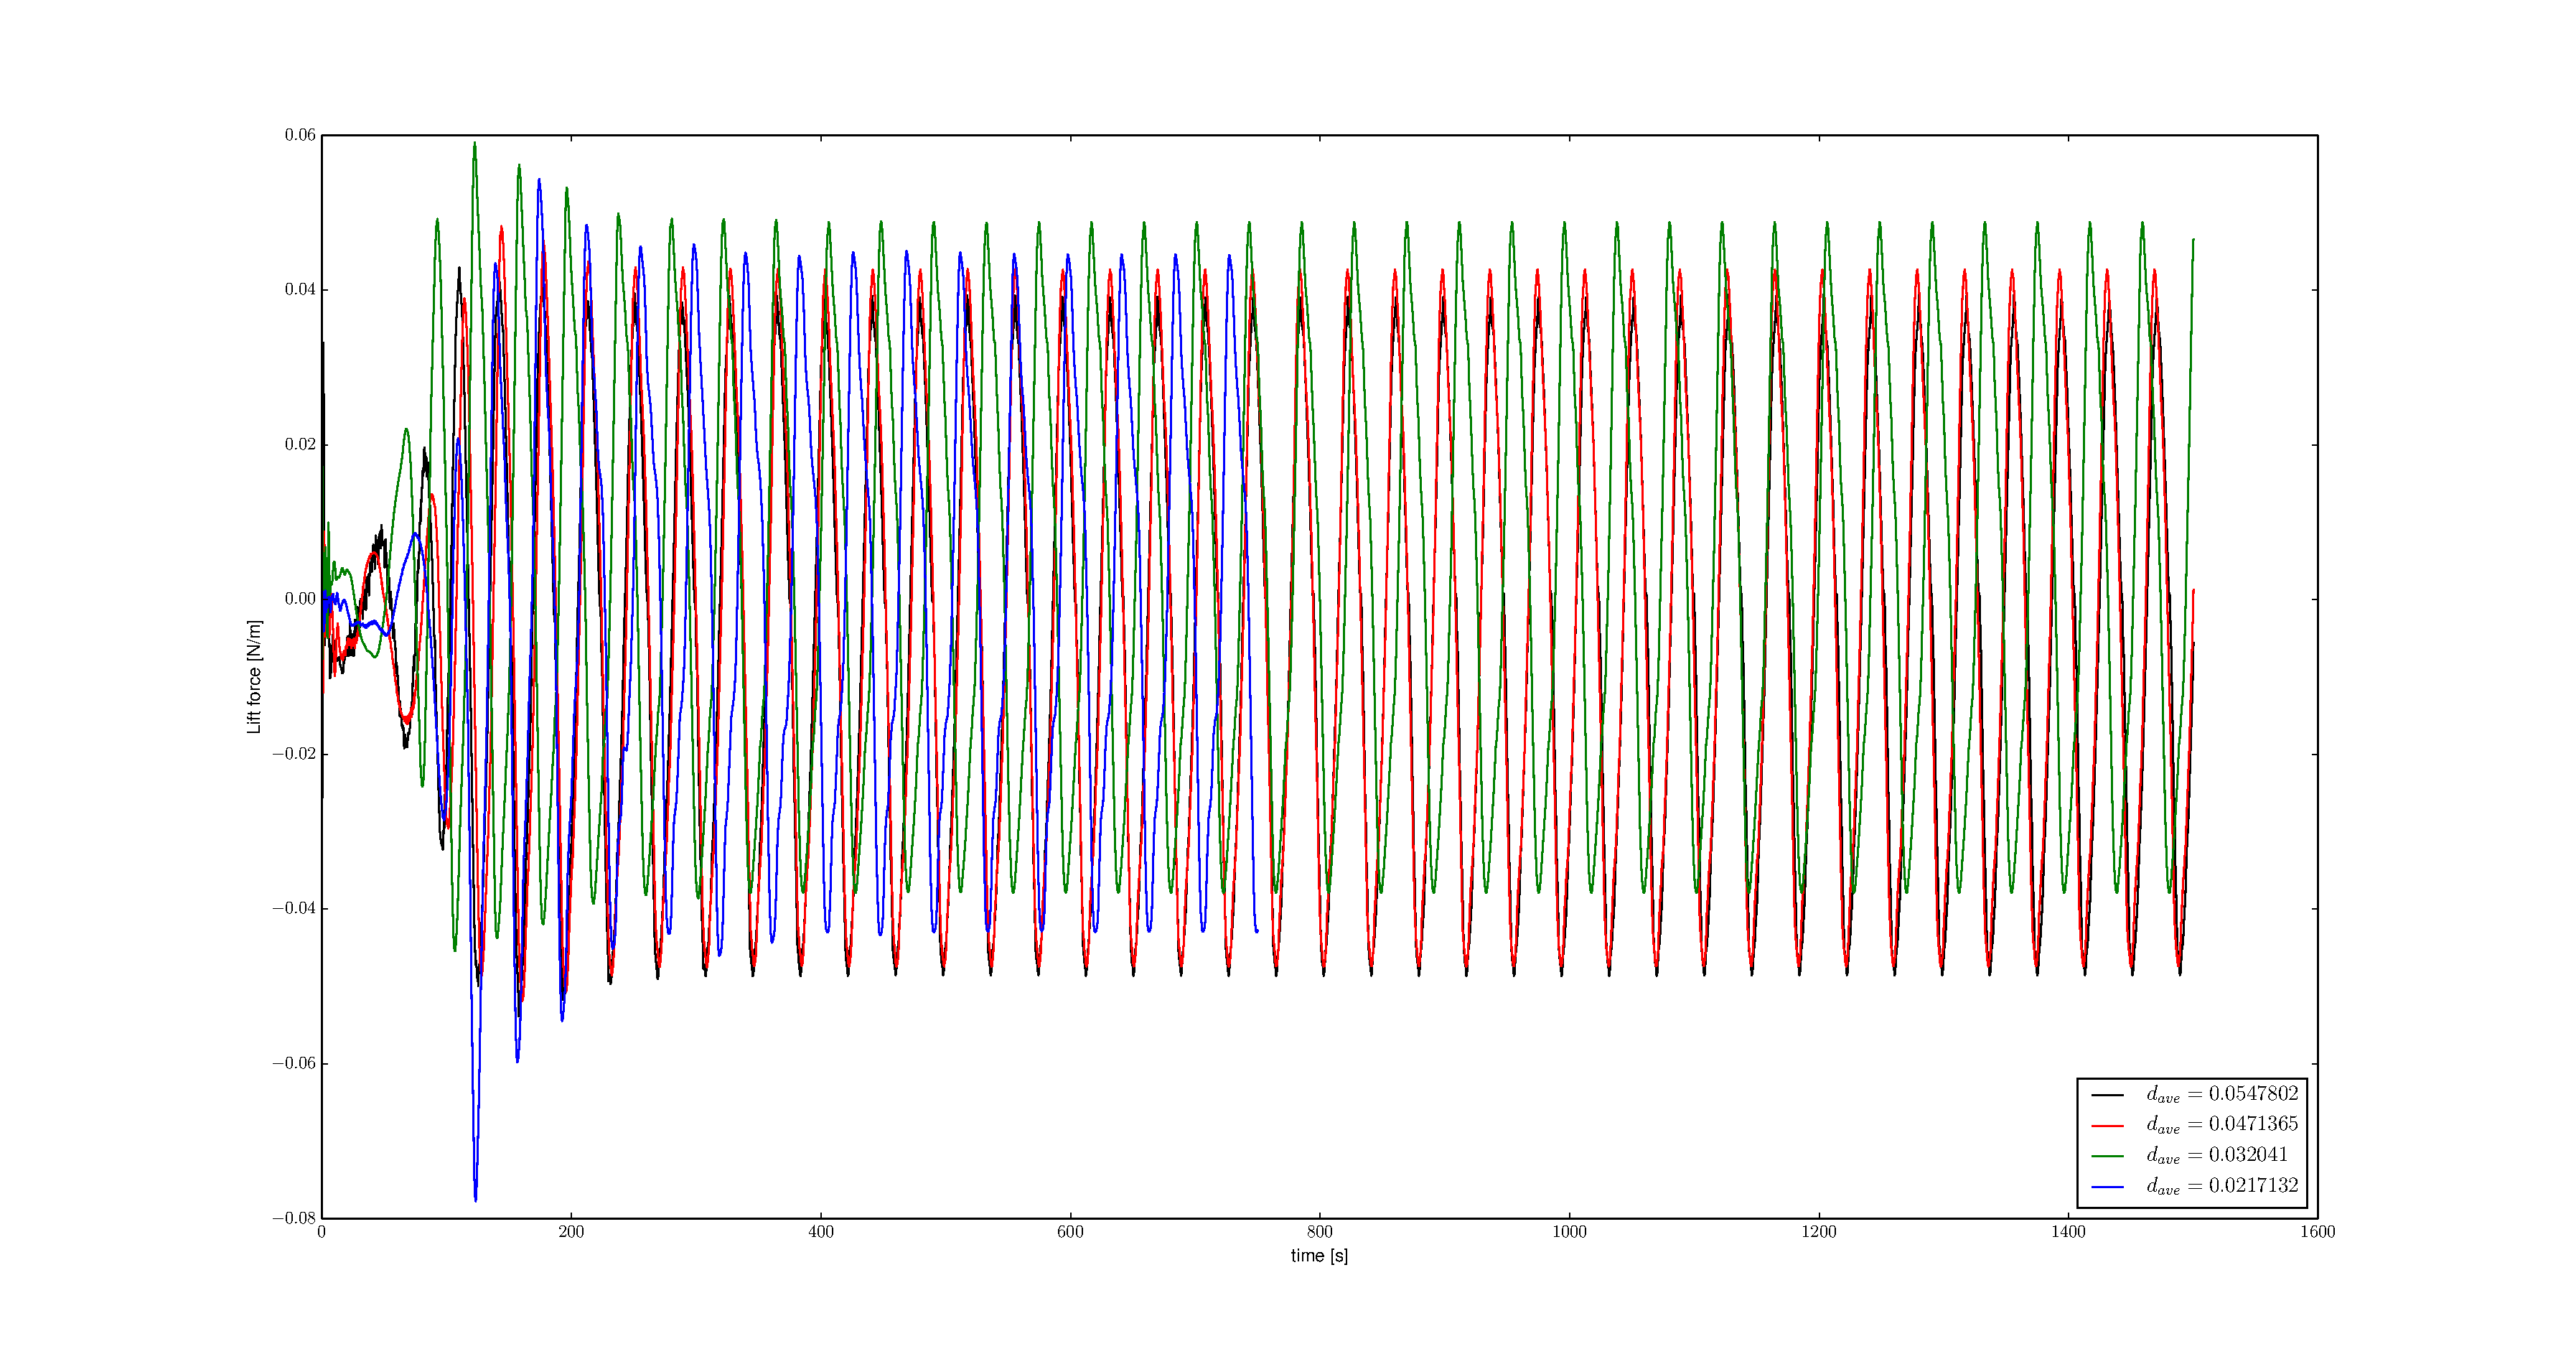
\includegraphics[width=\textwidth]{ForceTime.pdf}
			\caption{Lift force time history}
		\end{figure}

		\begin{figure}[H]
			\centering
			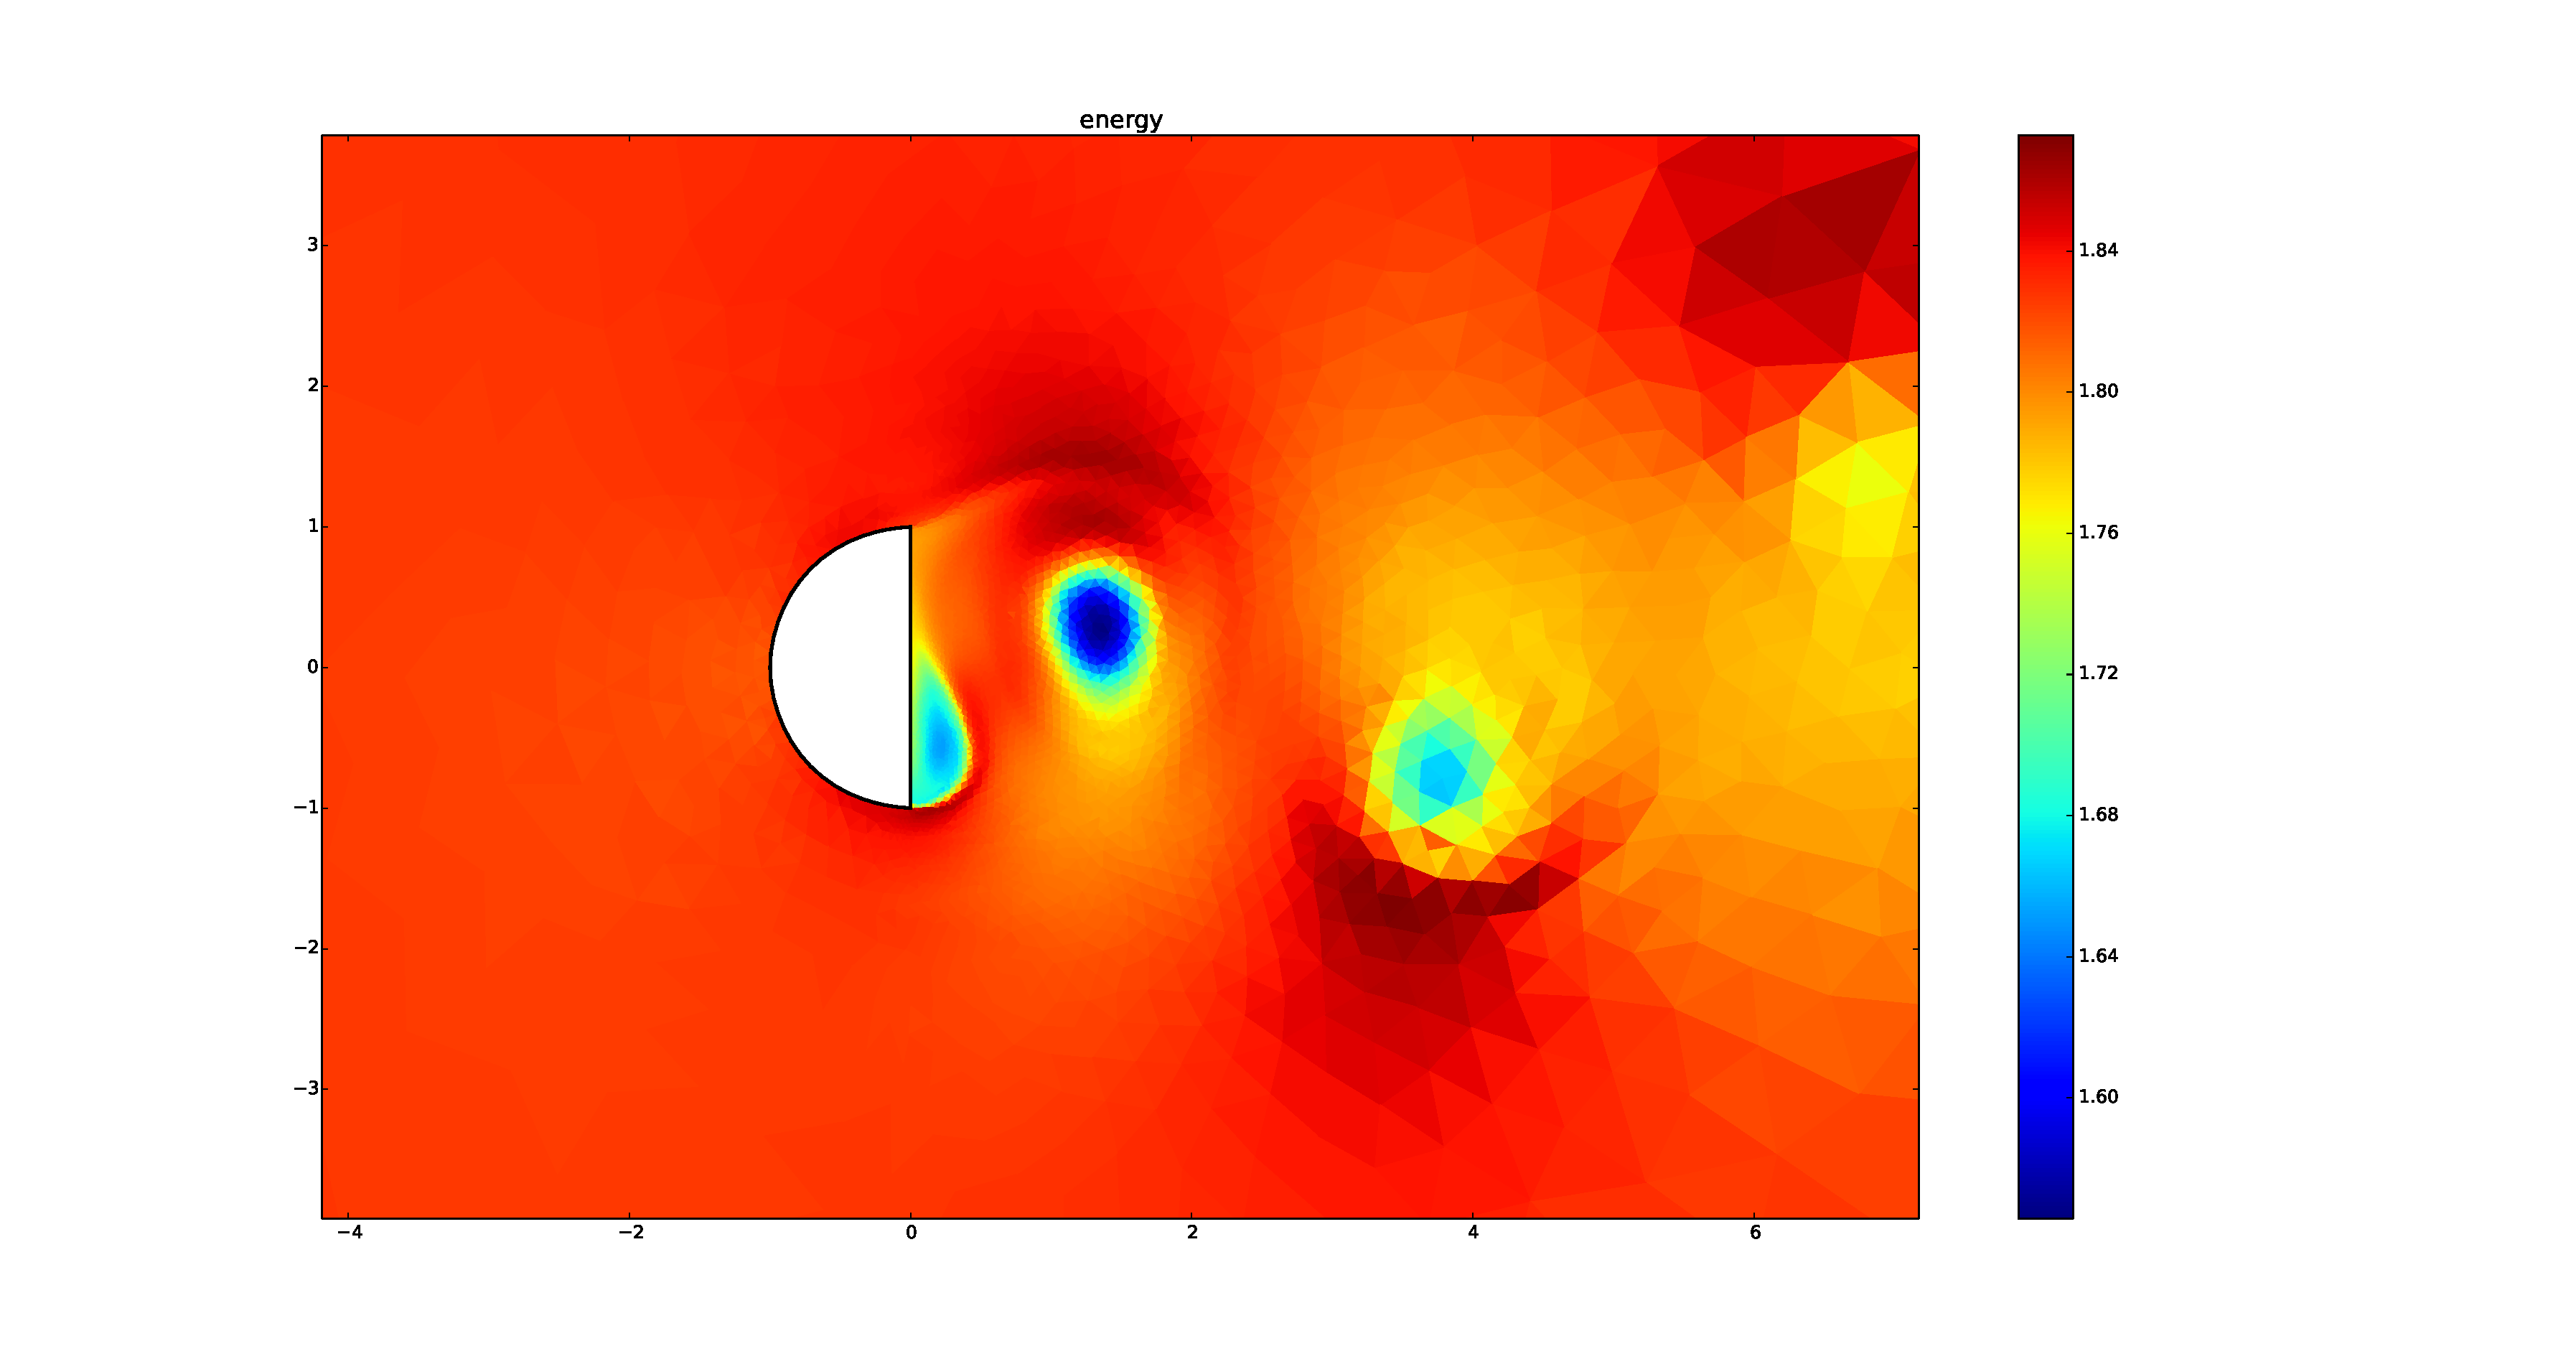
\includegraphics[width=\textwidth,trim={7cm 2cm 10cm 2cm},clip]{HalfCylinderVortex.pdf}
			\caption{A sample half cylinder shedding vortices}
		\end{figure}

		\bibliographystyle{siam}
		\bibliography{siam_sjoce335_A2163}
\end{document}
